\documentclass[crop,tikz]{standalone}

\usepackage{tikz}
\usetikzlibrary{patterns}

\pgfdeclarepatternformonly{south west lines}{\pgfqpoint{-0pt}{-0pt}}{\pgfqpoint{3pt}{3pt}}{\pgfqpoint{3pt}{3pt}}{
  \pgfsetlinewidth{0.4pt}
  \pgfpathmoveto{\pgfqpoint{0pt}{0pt}}
  \pgfpathlineto{\pgfqpoint{3pt}{3pt}}
  \pgfpathmoveto{\pgfqpoint{2.8pt}{-.2pt}}
  \pgfpathlineto{\pgfqpoint{3.2pt}{.2pt}}
  \pgfpathmoveto{\pgfqpoint{-.2pt}{2.8pt}}
  \pgfpathlineto{\pgfqpoint{.2pt}{3.2pt}}
  \pgfusepath{stroke}}

\pgfdeclarepatternformonly{south east lines}{\pgfqpoint{-0pt}{-0pt}}{\pgfqpoint{3pt}{3pt}}{\pgfqpoint{3pt}{3pt}}{
  \pgfsetlinewidth{0.4pt}
  \pgfpathmoveto{\pgfqpoint{0pt}{3pt}}
  \pgfpathlineto{\pgfqpoint{3pt}{0pt}}
  \pgfpathmoveto{\pgfqpoint{.2pt}{-.2pt}}
  \pgfpathlineto{\pgfqpoint{-.2pt}{.2pt}}
  \pgfpathmoveto{\pgfqpoint{3.2pt}{2.8pt}}
  \pgfpathlineto{\pgfqpoint{2.8pt}{3.2pt}}
  \pgfusepath{stroke}}

\begin{document}
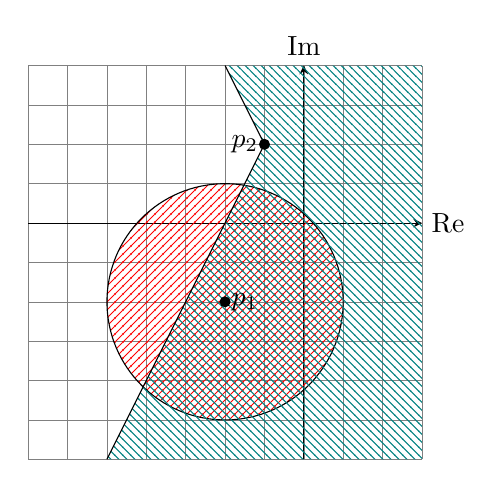
\begin{tikzpicture}[x=.5cm,y=.5cm]
  \draw[step=1, gray, very thin] (-7,-6) grid (3,4);
  \draw[-stealth] (-7,0)--(3,0) node[right]{Re}; % x axis
  \draw[-stealth] (0,-6)--(0,4) node[above]{Im}; % y axis

  \draw[pattern=south west lines, pattern color=red] (-2,-2) circle[radius=3];

  \fill[pattern=south east lines, pattern color=teal]
    (3,4)--(3,2)--(-1,2)--(-2,4)--cycle;
  \fill[pattern=south east lines, pattern color=teal]
    (3,-6)--(3,2)--(-1,2)--(-5,-6)--cycle;
  \draw (-2,4)--(-1,2)--(-5,-6);

  \node (a) at (-2,-2) {$\hspace{.5cm}p_1$};
  \node (b) at (-1,2) {$\hspace{-.5cm}p_2$};

  \fill (a) circle[radius=2pt];
  \fill (b) circle[radius=2pt];
\end{tikzpicture}
\end{document}
